% --------------------------------------------------------------
% This is all preamble stuff that you don't have to worry about.
% Head down to where it says "Start here"
% --------------------------------------------------------------
 
\documentclass[12pt]{article}
 
\usepackage[margin=1in]{geometry} 
\usepackage{amsmath,amsthm,amssymb}
 \usepackage{graphicx, color}
\newcommand{\N}{\mathbb{N}}
\newcommand{\Z}{\mathbb{Z}}
 
\newenvironment{theorem}[2][Theorem]{\begin{trivlist}
\item[\hskip \labelsep {\bfseries #1}\hskip \labelsep {\bfseries #2.}]}{\end{trivlist}}
\newenvironment{lemma}[2][Lemma]{\begin{trivlist}
\item[\hskip \labelsep {\bfseries #1}\hskip \labelsep {\bfseries #2.}]}{\end{trivlist}}
\newenvironment{exercise}[2][Exercise]{\begin{trivlist}
\item[\hskip \labelsep {\bfseries #1}\hskip \labelsep {\bfseries #2.}]}{\end{trivlist}}
\newenvironment{reflection}[2][Reflection]{\begin{trivlist}
\item[\hskip \labelsep {\bfseries #1}\hskip \labelsep {\bfseries #2.}]}{\end{trivlist}}
\newenvironment{proposition}[2][Proposition]{\begin{trivlist}
\item[\hskip \labelsep {\bfseries #1}\hskip \labelsep {\bfseries #2.}]}{\end{trivlist}}
\newenvironment{corollary}[2][Corollary]{\begin{trivlist}
\item[\hskip \labelsep {\bfseries #1}\hskip \labelsep {\bfseries #2.}]}{\end{trivlist}}
 
\begin{document}
 
% --------------------------------------------------------------
%                         Start here
% --------------------------------------------------------------
 
%\renewcommand{\qedsymbol}{\filledbox}
 
\title{Programming Assignment 2}%replace X with the appropriate number
\author{Sneha Reddy Aenugu, EE11B059\\ %replace with your name
} %if necessary, replace with your course title
 
\maketitle

\section{Backpropagation}
 
\begin{itemize}
\item{
For the implementation of backpropagation, stochastic gradient descent version of algorithm is used. The structure of the graph implemented is described in Table 1.

\begin{table}
\centering
		\begin{tabular}{|l | r|}
			\hline
			\textbf{Parameter} & \textbf{Value} \\ \hline
			 Number of layers & 3 \\ \hline
			Number of nodes in the input layer & 97 \\ \hline
			Number of nodes in the hidden layer & 50  \\ \hline
			Number of nodes in the output layer  & 4\\ \hline
			Activation function for the hidden layer  & Sigmoid function\\ \hline
			Activation function for the output layer  & Linear function\\ \hline
			Learning rate & 0.06 \\ \hline
			
			
			
		\end{tabular}
	\caption{Structure of the Neural Network}

\end{table}

The graph of Sum Squared Error versus the number of iterations is given in Figure 1.
\begin{figure}
	\centering
		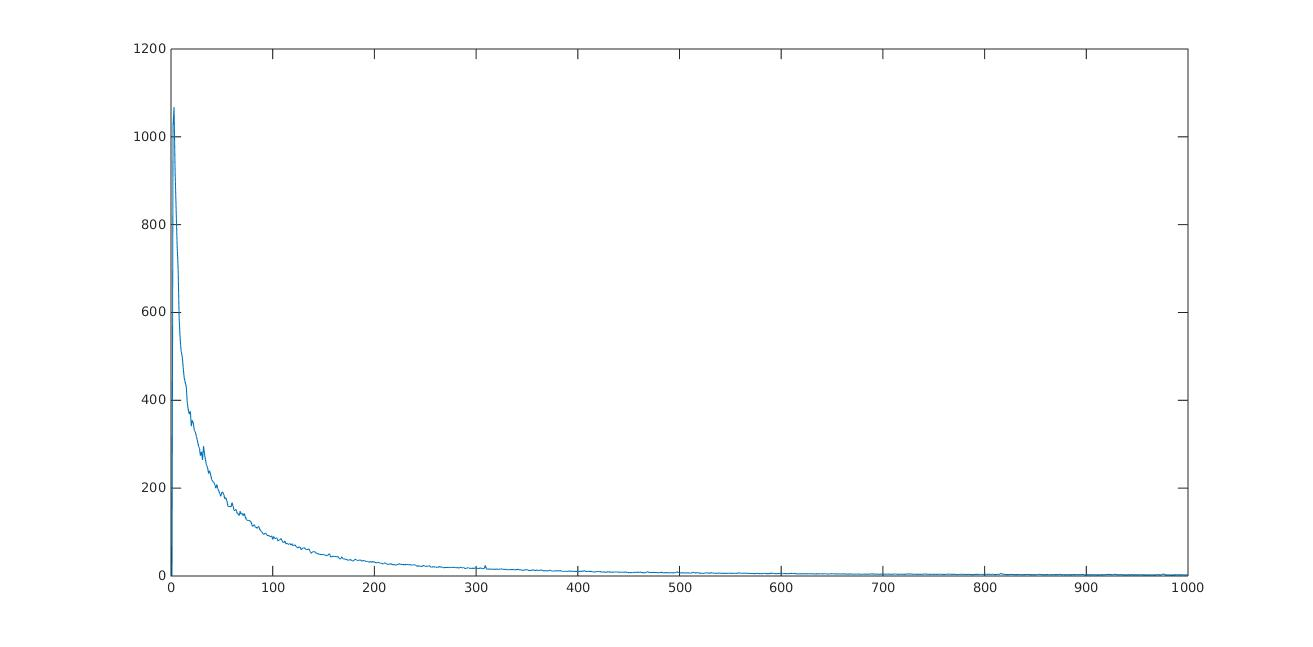
\includegraphics[scale = 0.4]{/home/sneha/Acads/9thsem/ML/P2/img1.jpg}
	\caption{Sum squared error plot vs iterations}
	
\end{figure}

\begin{equation}
Confusion\ Matrix = \begin{bmatrix} 17  & 1 & 1 & 1\\ 2 & 7 & 4 & 8 \\ 1 & 0 & 11 & 9 \\ 3 & 4 & 2 & 12 \end{bmatrix}
\end{equation}
Class 1:

\begin{equation}
Precision = 0.7391
\end{equation}
\begin{equation}
Recall = 0.85
\end{equation}
\begin{equation}
f-measure = 2*\frac{Precision*Recall}{Precision + Recall} = 0.7907
\end{equation}
\begin{equation}
Accuracy = 0.8916
\end{equation}

Class 2:

\begin{equation}
Precision = 0.5833
\end{equation}
\begin{equation}
Recall = 0.3333
\end{equation}
\begin{equation}
f-measure = 2*\frac{Precision*Recall}{Precision + Recall} = 0.4242
\end{equation}
\begin{equation}
Accuracy = 0.7711
\end{equation}

Class 3:

\begin{equation}
Precision = 0.6111
\end{equation}
\begin{equation}
Recall = 0.5238
\end{equation}
\begin{equation}
f-measure = 2*\frac{Precision*Recall}{Precision + Recall} = 0.5641
\end{equation}
\begin{equation}
Accuracy = 0.7952
\end{equation}

Class 4:

\begin{equation}
Precision = 0.40
\end{equation}
\begin{equation}
Recall = 0.5714
\end{equation}
\begin{equation}
f-measure = 2*\frac{Precision*Recall}{Precision + Recall} = 0.4706
\end{equation}
\begin{equation}
Accuracy = 0.6747
\end{equation}

}
\item{
With regularization, the gradient descent update rule changes as shown below.

\begin{equation}
w = w +  \delta w - \nu * \lambda * w
\end{equation}

where $w$ = weights to be updated, $\nu$ = learning rate, $\lambda$ = regularization factor.\\

The plot of Sum Squared error versus the iterations is given in the Figure 2.

\begin{figure}
	\centering
		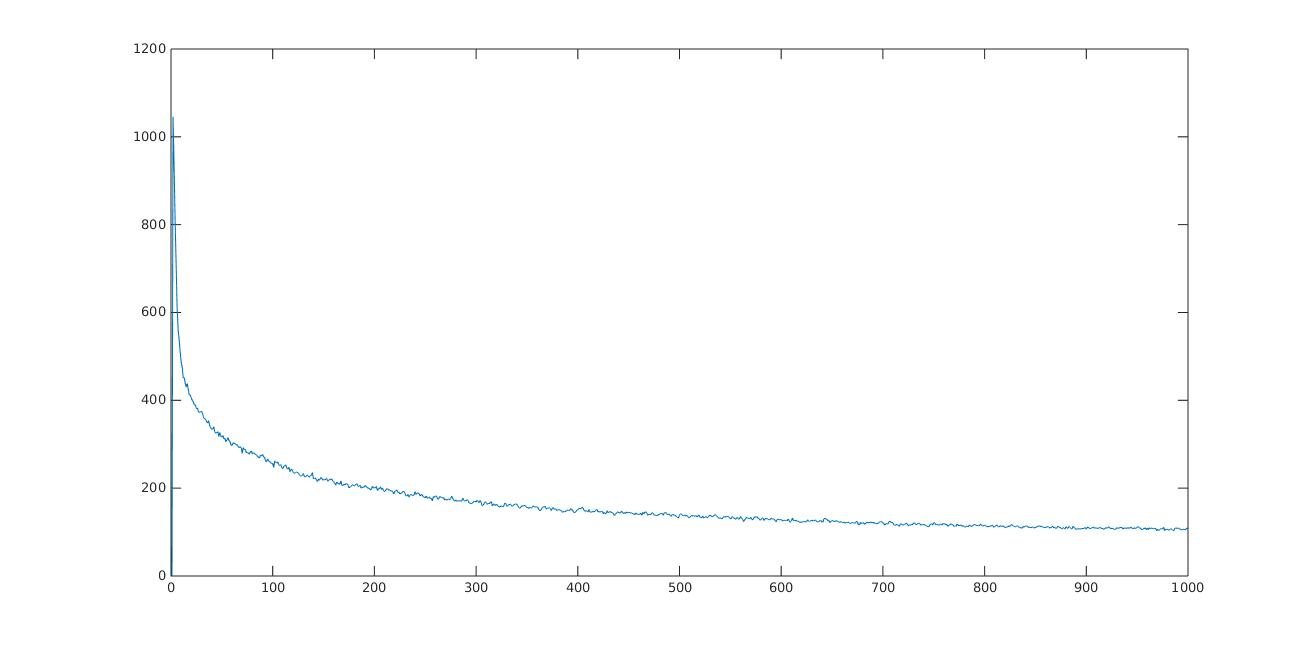
\includegraphics[scale = 0.4]{/home/sneha/Acads/9thsem/ML/P2/img12.jpg}
	\caption{Sum squared error plot vs iterations}
	
\end{figure}

\begin{equation}
Confusion\ Matrix = \begin{bmatrix} 17  & 1 & 2 & 0\\ 0 & 11 & 5 & 5 \\ 2 & 0 & 19 & 0 \\ 2 & 6 & 5 & 8 \end{bmatrix}
\end{equation}
Class 1:

\begin{equation}
Precision = 0.8095
\end{equation}
\begin{equation}
Recall = 0.8500
\end{equation}
\begin{equation}
f-measure = 2*\frac{Precision*Recall}{Precision + Recall} = 0.8293
\end{equation}
\begin{equation}
Accuracy = 0.9157
\end{equation}

Class 2:

\begin{equation}
Precision = 0.6111
\end{equation}
\begin{equation}
Recall = 0.5238
\end{equation}
\begin{equation}
f-measure = 2*\frac{Precision*Recall}{Precision + Recall} = 0.5641
\end{equation}
\begin{equation}
Accuracy = 0.7952
\end{equation}

Class 3:

\begin{equation}
Precision = 0.6129
\end{equation}
\begin{equation}
Recall = 0.9048
\end{equation}
\begin{equation}
f-measure = 2*\frac{Precision*Recall}{Precision + Recall} = 0.7308
\end{equation}
\begin{equation}
Accuracy = 0.8313
\end{equation}

Class 4:

\begin{equation}
Precision = 0.6154
\end{equation}
\begin{equation}
Recall = 0.3810
\end{equation}
\begin{equation}
f-measure = 2*\frac{Precision*Recall}{Precision + Recall} = 0.4706
\end{equation}
\begin{equation}
Accuracy = 0.7831
\end{equation}


With regularization, there is an improvement in the classification accuracy, precision and recall. As $\lambda$ (regularization factor increases) the classification is inaccurate as the weights are too constrained.
}




\end{itemize}




\section{QDA \& RDA}

For the purpose of this problem, only petal length and petal width features are considered. The decision boundaries for LDA, QDA and RDA are shown in Figure 2, Figure 3 and Figure 4 respectively.


\begin{figure}


	\centering
		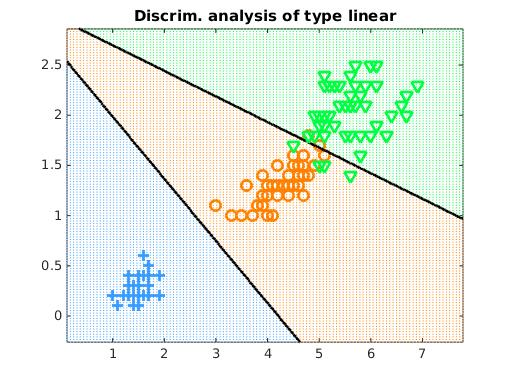
\includegraphics[scale = 0.7]{/home/sneha/Acads/9thsem/ML/P2/img31.jpg}
	\caption{Decision boundaries for LDA}
	
\end{figure}


\begin{figure}
	\centering
		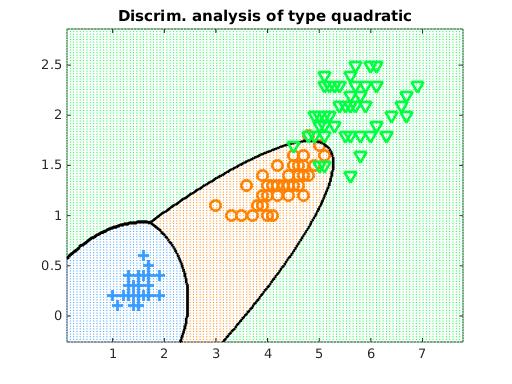
\includegraphics[scale = 0.7]{/home/sneha/Acads/9thsem/ML/P2/img32.jpg}
	\caption{Decision boundaries for QDA}
	
\end{figure}

\begin{figure}
	\centering
		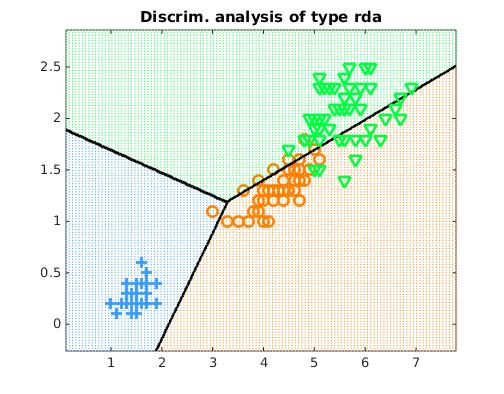
\includegraphics[scale = 0.7]{/home/sneha/Acads/9thsem/ML/P2/img33.jpg}
	\caption{Decision boundaries for RDA}
	
\end{figure}









\section{Logistic Regression}

For the purpose of this problem a one vs all classifer procedure is used. 
\subsection{Logistic Regression}

The confusion matrices, precision, recall, f- measure values are given below for logistic regression of classification of DS4.\\
\\
\textbf{Class 1:}

\begin{equation} 
Confusion\ Matrix = \begin{bmatrix} 8  & 12 \\ 4 & 59 \end{bmatrix}
\end{equation}

\begin{equation}
Precision = 0.6667
\end{equation}
\begin{equation}
Recall = 0.40
\end{equation}
\begin{equation}
f-measure = 2*\frac{Precision*Recall}{Precision + Recall} = 0.8512
\end{equation}


\textbf{Class 2:}
\begin{equation}
Confusion\ Matrix = \begin{bmatrix} 11  & 10 \\ 5 & 57 \end{bmatrix}
\end{equation}
\begin{equation}
Precision = 0.6875
\end{equation}
\begin{equation}
Recall = 0.5238
\end{equation}
\begin{equation}
f-measure = 2*\frac{Precision*Recall}{Precision + Recall} = 0.8054
\end{equation}


\textbf{Class 3:}
\begin{equation}
Confusion\ Matrix = \begin{bmatrix} 16 & 5 \\ 6 & 56 \end{bmatrix}
\end{equation}
\begin{equation}
Precision = 0.7273
\end{equation}
\begin{equation}
Recall = 0.7619
\end{equation}
\begin{equation}
f-measure = 2*\frac{Precision*Recall}{Precision + Recall} = 0.7336
\end{equation}


\textbf{Class 4:}
\begin{equation}
Confusion\ Matrix = \begin{bmatrix} 16  & 5 \\ 2 & 60 \end{bmatrix}
\end{equation}
\begin{equation}
Precision = 0.8889
\end{equation}
\begin{equation}
Recall = 0.7619
\end{equation}
\begin{equation}
f-measure = 2*\frac{Precision*Recall}{Precision + Recall} = 0.7059
\end{equation}


\subsection{Regularized Logistic Regression}

The confusion matrices, precision, recall, f- measure values are given below for one vs rest method of classification. The $\lambda$ value chosen for the regularization is $0.1$. 
\\
\\
\textbf{Class 1:}

\begin{equation}
Confusion\ Matrix = \begin{bmatrix} 7  & 13 \\ 1 & 62 \end{bmatrix}
\end{equation}

\begin{equation}
Precision = 0.8750
\end{equation}
\begin{equation}
Recall = 0.35
\end{equation}
\begin{equation}
f-measure = 2*\frac{Precision*Recall}{Precision + Recall} = 0.7460
\end{equation}


\textbf{Class 2:}
\begin{equation}
Confusion\ Matrix = \begin{bmatrix} 16  & 5 \\ 0 & 62 \end{bmatrix}
\end{equation}
\begin{equation}
Precision = 1
\end{equation}
\begin{equation}
Recall = 0.7619
\end{equation}
\begin{equation}
f-measure = 2*\frac{Precision*Recall}{Precision + Recall} = 0.7460
\end{equation}


\textbf{Class 3:}
\begin{equation}
Confusion\ Matrix = \begin{bmatrix} 20  & 1 \\ 2 & 60 \end{bmatrix}
\end{equation}
\begin{equation}
Precision = 0.9091
\end{equation}
\begin{equation}
Recall = 0.9524
\end{equation}
\begin{equation}
f-measure = 2*\frac{Precision*Recall}{Precision + Recall} = 0.8251
\end{equation}


\textbf{Class 4:}
\begin{equation}
Confusion\ Matrix = \begin{bmatrix} 18  & 3 \\ 2 & 60 \end{bmatrix}
\end{equation}
\begin{equation}
Precision = 0.90
\end{equation}
\begin{equation}
Recall = 0.8571
\end{equation}
\begin{equation}
f-measure = 2*\frac{Precision*Recall}{Precision + Recall} = 0.8397
\end{equation}
With regularization, there is a huge improvement in the classification accuracy, precision and recall.



% --------------------------------------------------------------
%     You don't have to mess with anything below this line.
% --------------------------------------------------------------
 
\end{document}